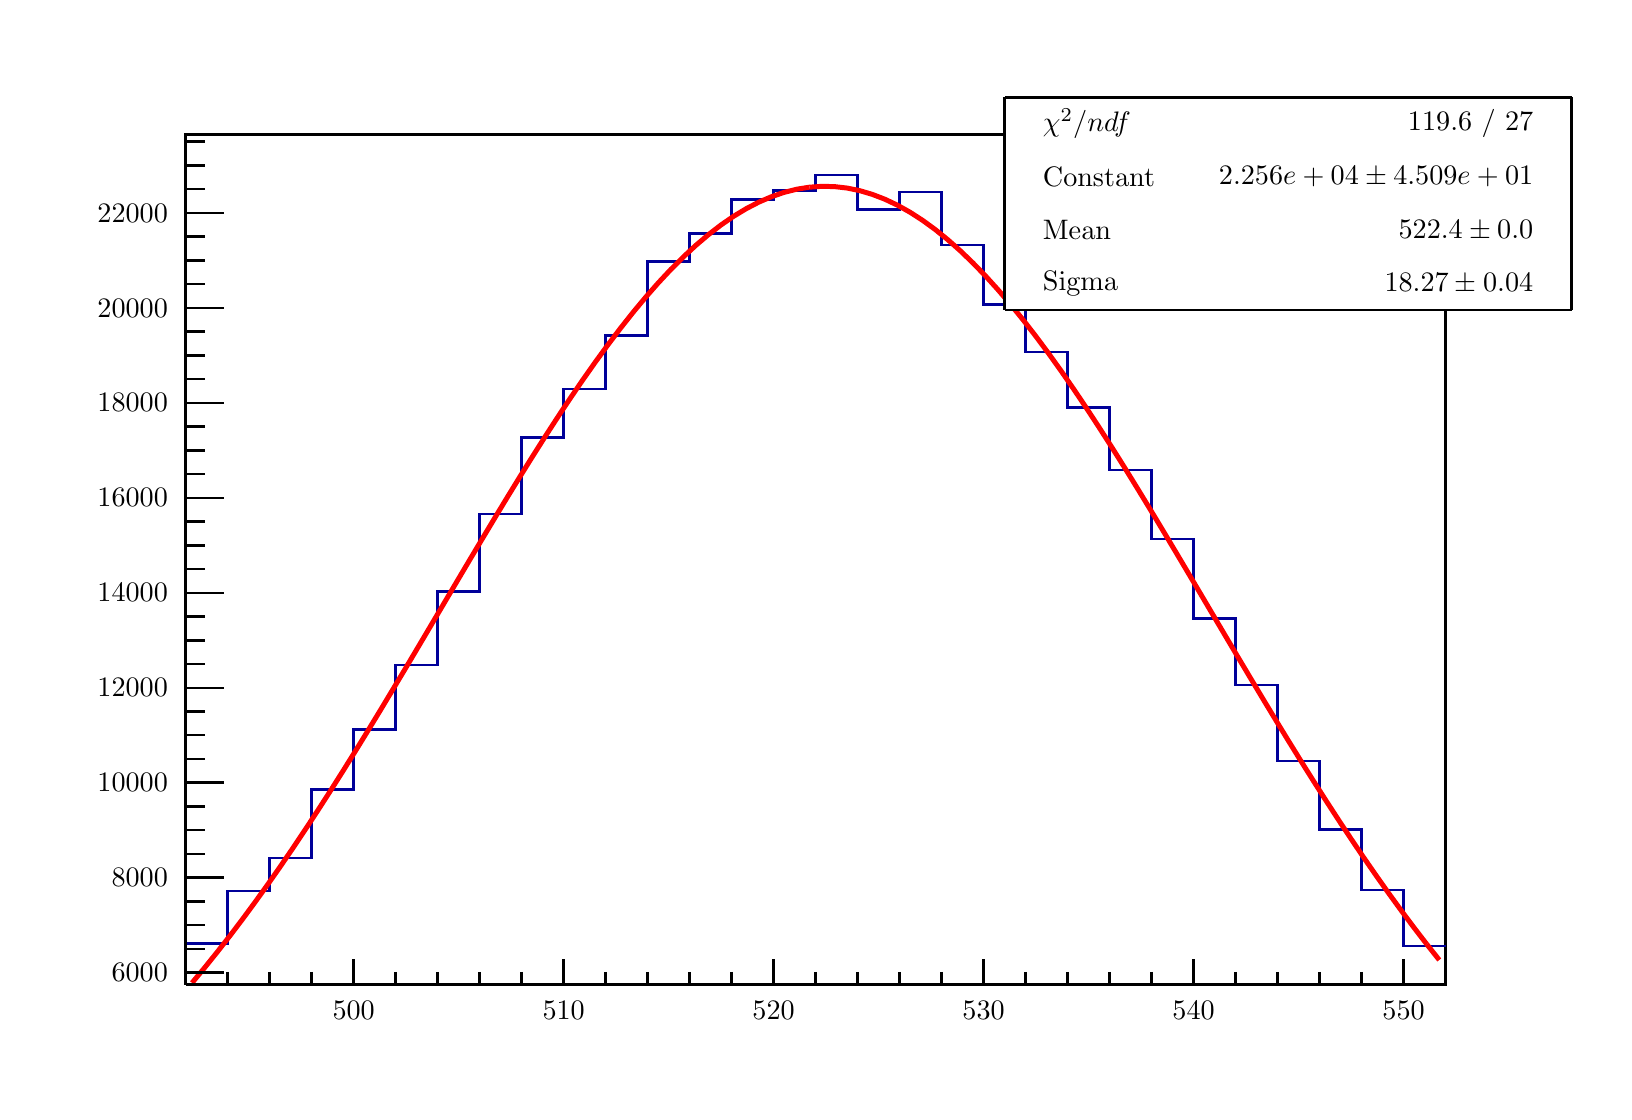
\begin{tikzpicture}
\pgfdeclareplotmark{cross} {
\pgfpathmoveto{\pgfpoint{-0.3\pgfplotmarksize}{\pgfplotmarksize}}
\pgfpathlineto{\pgfpoint{+0.3\pgfplotmarksize}{\pgfplotmarksize}}
\pgfpathlineto{\pgfpoint{+0.3\pgfplotmarksize}{0.3\pgfplotmarksize}}
\pgfpathlineto{\pgfpoint{+1\pgfplotmarksize}{0.3\pgfplotmarksize}}
\pgfpathlineto{\pgfpoint{+1\pgfplotmarksize}{-0.3\pgfplotmarksize}}
\pgfpathlineto{\pgfpoint{+0.3\pgfplotmarksize}{-0.3\pgfplotmarksize}}
\pgfpathlineto{\pgfpoint{+0.3\pgfplotmarksize}{-1.\pgfplotmarksize}}
\pgfpathlineto{\pgfpoint{-0.3\pgfplotmarksize}{-1.\pgfplotmarksize}}
\pgfpathlineto{\pgfpoint{-0.3\pgfplotmarksize}{-0.3\pgfplotmarksize}}
\pgfpathlineto{\pgfpoint{-1.\pgfplotmarksize}{-0.3\pgfplotmarksize}}
\pgfpathlineto{\pgfpoint{-1.\pgfplotmarksize}{0.3\pgfplotmarksize}}
\pgfpathlineto{\pgfpoint{-0.3\pgfplotmarksize}{0.3\pgfplotmarksize}}
\pgfpathclose
\pgfusepathqstroke
}
\pgfdeclareplotmark{cross*} {
\pgfpathmoveto{\pgfpoint{-0.3\pgfplotmarksize}{\pgfplotmarksize}}
\pgfpathlineto{\pgfpoint{+0.3\pgfplotmarksize}{\pgfplotmarksize}}
\pgfpathlineto{\pgfpoint{+0.3\pgfplotmarksize}{0.3\pgfplotmarksize}}
\pgfpathlineto{\pgfpoint{+1\pgfplotmarksize}{0.3\pgfplotmarksize}}
\pgfpathlineto{\pgfpoint{+1\pgfplotmarksize}{-0.3\pgfplotmarksize}}
\pgfpathlineto{\pgfpoint{+0.3\pgfplotmarksize}{-0.3\pgfplotmarksize}}
\pgfpathlineto{\pgfpoint{+0.3\pgfplotmarksize}{-1.\pgfplotmarksize}}
\pgfpathlineto{\pgfpoint{-0.3\pgfplotmarksize}{-1.\pgfplotmarksize}}
\pgfpathlineto{\pgfpoint{-0.3\pgfplotmarksize}{-0.3\pgfplotmarksize}}
\pgfpathlineto{\pgfpoint{-1.\pgfplotmarksize}{-0.3\pgfplotmarksize}}
\pgfpathlineto{\pgfpoint{-1.\pgfplotmarksize}{0.3\pgfplotmarksize}}
\pgfpathlineto{\pgfpoint{-0.3\pgfplotmarksize}{0.3\pgfplotmarksize}}
\pgfpathclose
\pgfusepathqfillstroke
}
\pgfdeclareplotmark{newstar} {
\pgfpathmoveto{\pgfqpoint{0pt}{\pgfplotmarksize}}
\pgfpathlineto{\pgfqpointpolar{44}{0.5\pgfplotmarksize}}
\pgfpathlineto{\pgfqpointpolar{18}{\pgfplotmarksize}}
\pgfpathlineto{\pgfqpointpolar{-20}{0.5\pgfplotmarksize}}
\pgfpathlineto{\pgfqpointpolar{-54}{\pgfplotmarksize}}
\pgfpathlineto{\pgfqpointpolar{-90}{0.5\pgfplotmarksize}}
\pgfpathlineto{\pgfqpointpolar{234}{\pgfplotmarksize}}
\pgfpathlineto{\pgfqpointpolar{198}{0.5\pgfplotmarksize}}
\pgfpathlineto{\pgfqpointpolar{162}{\pgfplotmarksize}}
\pgfpathlineto{\pgfqpointpolar{134}{0.5\pgfplotmarksize}}
\pgfpathclose
\pgfusepathqstroke
}
\pgfdeclareplotmark{newstar*} {
\pgfpathmoveto{\pgfqpoint{0pt}{\pgfplotmarksize}}
\pgfpathlineto{\pgfqpointpolar{44}{0.5\pgfplotmarksize}}
\pgfpathlineto{\pgfqpointpolar{18}{\pgfplotmarksize}}
\pgfpathlineto{\pgfqpointpolar{-20}{0.5\pgfplotmarksize}}
\pgfpathlineto{\pgfqpointpolar{-54}{\pgfplotmarksize}}
\pgfpathlineto{\pgfqpointpolar{-90}{0.5\pgfplotmarksize}}
\pgfpathlineto{\pgfqpointpolar{234}{\pgfplotmarksize}}
\pgfpathlineto{\pgfqpointpolar{198}{0.5\pgfplotmarksize}}
\pgfpathlineto{\pgfqpointpolar{162}{\pgfplotmarksize}}
\pgfpathlineto{\pgfqpointpolar{134}{0.5\pgfplotmarksize}}
\pgfpathclose
\pgfusepathqfillstroke
}
\definecolor{c}{rgb}{1,1,1};
\draw [color=c, fill=c] (0,0) rectangle (20,13.4957);
\draw [color=c, fill=c] (2,1.34957) rectangle (18,12.1461);
\definecolor{c}{rgb}{0,0,0};
\draw [c,line width=0.9] (2,1.34957) -- (2,12.1461) -- (18,12.1461) -- (18,1.34957) -- (2,1.34957);
\definecolor{c}{rgb}{1,1,1};
\draw [color=c, fill=c] (2,1.34957) rectangle (18,12.1461);
\definecolor{c}{rgb}{0,0,0};
\draw [c,line width=0.9] (2,1.34957) -- (2,12.1461) -- (18,12.1461) -- (18,1.34957) -- (2,1.34957);
\definecolor{c}{rgb}{0,0,0.6};
\draw [c,line width=0.9] (2,1.87057) -- (2.53333,1.87057) -- (2.53333,2.5399) -- (3.06667,2.5399) -- (3.06667,2.95658) -- (3.6,2.95658) -- (3.6,3.82792) -- (4.13333,3.82792) -- (4.13333,4.58831) -- (4.66667,4.58831) -- (4.66667,5.40659) --
 (5.2,5.40659) -- (5.2,6.34305) -- (5.73333,6.34305) -- (5.73333,7.32354) -- (6.26667,7.32354) -- (6.26667,8.298) -- (6.8,8.298) -- (6.8,8.91608) -- (7.33333,8.91608) -- (7.33333,9.59265) -- (7.86667,9.59265) -- (7.86667,10.5339) -- (8.4,10.5339) --
 (8.4,10.8915) -- (8.93333,10.8915) -- (8.93333,11.3209) -- (9.46667,11.3209) -- (9.46667,11.4342) -- (10,11.4342) -- (10,11.632) -- (10.5333,11.632) -- (10.5333,11.1942) -- (11.0667,11.1942) -- (11.0667,11.4125) -- (11.6,11.4125) -- (11.6,10.7444)
 -- (12.1333,10.7444) -- (12.1333,9.98822) -- (12.6667,9.98822) -- (12.6667,9.3822) -- (13.2,9.3822) -- (13.2,8.67668) -- (13.7333,8.67668) -- (13.7333,7.88675) -- (14.2667,7.88675) -- (14.2667,7.01179) -- (14.8,7.01179) -- (14.8,6.00175) --
 (15.3333,6.00175) -- (15.3333,5.15152) -- (15.8667,5.15152) -- (15.8667,4.19093) -- (16.4,4.19093) -- (16.4,3.32019) -- (16.9333,3.32019) -- (16.9333,2.55136) -- (17.4667,2.55136) -- (17.4667,1.83921) -- (18,1.83921);
\definecolor{c}{rgb}{1,1,1};
\draw [color=c, fill=c] (12.4,9.91934) rectangle (19.6,12.6185);
\definecolor{c}{rgb}{0,0,0};
\draw [c,line width=0.9] (12.4,9.91934) -- (19.6,9.91934);
\draw [c,line width=0.9] (19.6,9.91934) -- (19.6,12.6185);
\draw [c,line width=0.9] (19.6,12.6185) -- (12.4,12.6185);
\draw [c,line width=0.9] (12.4,12.6185) -- (12.4,9.91934);
\draw [anchor= west] (12.76,12.2811) node[scale=1.01821, color=c, rotate=0]{$\chi^{2} / ndf $};
\draw [anchor= east] (19.24,12.2811) node[scale=1.01821, color=c, rotate=0]{ 119.6 / 27};
\draw [anchor= west] (12.76,11.6063) node[scale=1.01821, color=c, rotate=0]{Constant };
\draw [anchor= east] (19.24,11.6063) node[scale=1.01821, color=c, rotate=0]{$ 2.256e+04 \pm 4.509e+01$};
\draw [anchor= west] (12.76,10.9315) node[scale=1.01821, color=c, rotate=0]{Mean     };
\draw [anchor= east] (19.24,10.9315) node[scale=1.01821, color=c, rotate=0]{$ 522.4 \pm 0.0$};
\draw [anchor= west] (12.76,10.2567) node[scale=1.01821, color=c, rotate=0]{Sigma    };
\draw [anchor= east] (19.24,10.2567) node[scale=1.01821, color=c, rotate=0]{$ 18.27 \pm 0.04$};
\definecolor{c}{rgb}{1,0,0};
\draw [c,line width=1.8] (2.08,1.3719) -- (2.24,1.56409) -- (2.4,1.76268) -- (2.56,1.96758) -- (2.72,2.17867) -- (2.88,2.39581) -- (3.04,2.61882) -- (3.2,2.84749) -- (3.36,3.0816) -- (3.52,3.32089) -- (3.68,3.56507) -- (3.84,3.81381) -- (4,4.06677)
 -- (4.16,4.32358) -- (4.32,4.58383) -- (4.48,4.84708) -- (4.64,5.11288) -- (4.8,5.38074) -- (4.96,5.65015) -- (5.12,5.92057) -- (5.28,6.19144) -- (5.44,6.46219) -- (5.6,6.73223) -- (5.76,7.00092) -- (5.92,7.26766) -- (6.08,7.53179) -- (6.24,7.79267)
 -- (6.4,8.04963) -- (6.56,8.30203) -- (6.72,8.54918) -- (6.88,8.79044) -- (7.04,9.02514) -- (7.2,9.25262) -- (7.36,9.47225) -- (7.52,9.68339) -- (7.68,9.88544) -- (7.84,10.0778) -- (8,10.2599) -- (8.16,10.4312) -- (8.32,10.5911) -- (8.48,10.7392) --
 (8.64,10.875) -- (8.8,10.9982) -- (8.96,11.1082) -- (9.12,11.2047) -- (9.28,11.2876) -- (9.44,11.3564) -- (9.6,11.4109) -- (9.76,11.4511) -- (9.92,11.4767);
\draw [c,line width=1.8] (9.92,11.4767) -- (10.08,11.4877) -- (10.24,11.484) -- (10.4,11.4657) -- (10.56,11.4328) -- (10.72,11.3854) -- (10.88,11.3237) -- (11.04,11.2478) -- (11.2,11.1581) -- (11.36,11.0547) -- (11.52,10.9381) -- (11.68,10.8086) --
 (11.84,10.6666) -- (12,10.5125) -- (12.16,10.3468) -- (12.32,10.17) -- (12.48,9.98274) -- (12.64,9.78546) -- (12.8,9.57878) -- (12.96,9.36331) -- (13.12,9.13967) -- (13.28,8.90849) -- (13.44,8.67043) -- (13.6,8.42614) -- (13.76,8.17628) --
 (13.92,7.92151) -- (14.08,7.6625) -- (14.24,7.39991) -- (14.4,7.1344) -- (14.56,6.8666) -- (14.72,6.59716) -- (14.88,6.32669) -- (15.04,6.05581) -- (15.2,5.78509) -- (15.36,5.51511) -- (15.52,5.24641) -- (15.68,4.97952) -- (15.84,4.71493) --
 (16,4.45313) -- (16.16,4.19455) -- (16.32,3.93962) -- (16.48,3.68872) -- (16.64,3.44222) -- (16.8,3.20046) -- (16.96,2.96373) -- (17.12,2.73231) -- (17.28,2.50645) -- (17.44,2.28635) -- (17.6,2.07222) -- (17.76,1.86421);
\draw [c,line width=1.8] (17.76,1.86421) -- (17.92,1.66246);
\definecolor{c}{rgb}{0,0,0};
\draw [c,line width=0.9] (2,1.34957) -- (18,1.34957);
\draw [c,line width=0.9] (4.13333,1.67347) -- (4.13333,1.34957);
\draw [c,line width=0.9] (4.66667,1.51152) -- (4.66667,1.34957);
\draw [c,line width=0.9] (5.2,1.51152) -- (5.2,1.34957);
\draw [c,line width=0.9] (5.73333,1.51152) -- (5.73333,1.34957);
\draw [c,line width=0.9] (6.26667,1.51152) -- (6.26667,1.34957);
\draw [c,line width=0.9] (6.8,1.67347) -- (6.8,1.34957);
\draw [c,line width=0.9] (7.33333,1.51152) -- (7.33333,1.34957);
\draw [c,line width=0.9] (7.86667,1.51152) -- (7.86667,1.34957);
\draw [c,line width=0.9] (8.4,1.51152) -- (8.4,1.34957);
\draw [c,line width=0.9] (8.93333,1.51152) -- (8.93333,1.34957);
\draw [c,line width=0.9] (9.46667,1.67347) -- (9.46667,1.34957);
\draw [c,line width=0.9] (10,1.51152) -- (10,1.34957);
\draw [c,line width=0.9] (10.5333,1.51152) -- (10.5333,1.34957);
\draw [c,line width=0.9] (11.0667,1.51152) -- (11.0667,1.34957);
\draw [c,line width=0.9] (11.6,1.51152) -- (11.6,1.34957);
\draw [c,line width=0.9] (12.1333,1.67347) -- (12.1333,1.34957);
\draw [c,line width=0.9] (12.6667,1.51152) -- (12.6667,1.34957);
\draw [c,line width=0.9] (13.2,1.51152) -- (13.2,1.34957);
\draw [c,line width=0.9] (13.7333,1.51152) -- (13.7333,1.34957);
\draw [c,line width=0.9] (14.2667,1.51152) -- (14.2667,1.34957);
\draw [c,line width=0.9] (14.8,1.67347) -- (14.8,1.34957);
\draw [c,line width=0.9] (15.3333,1.51152) -- (15.3333,1.34957);
\draw [c,line width=0.9] (15.8667,1.51152) -- (15.8667,1.34957);
\draw [c,line width=0.9] (16.4,1.51152) -- (16.4,1.34957);
\draw [c,line width=0.9] (16.9333,1.51152) -- (16.9333,1.34957);
\draw [c,line width=0.9] (17.4667,1.67347) -- (17.4667,1.34957);
\draw [c,line width=0.9] (4.13333,1.67347) -- (4.13333,1.34957);
\draw [c,line width=0.9] (3.6,1.51152) -- (3.6,1.34957);
\draw [c,line width=0.9] (3.06667,1.51152) -- (3.06667,1.34957);
\draw [c,line width=0.9] (2.53333,1.51152) -- (2.53333,1.34957);
\draw [c,line width=0.9] (17.4667,1.67347) -- (17.4667,1.34957);
\draw [c,line width=0.9] (18,1.51152) -- (18,1.34957);
\draw [anchor=base] (4.13333,0.904212) node[scale=1.01821, color=c, rotate=0]{500};
\draw [anchor=base] (6.8,0.904212) node[scale=1.01821, color=c, rotate=0]{510};
\draw [anchor=base] (9.46667,0.904212) node[scale=1.01821, color=c, rotate=0]{520};
\draw [anchor=base] (12.1333,0.904212) node[scale=1.01821, color=c, rotate=0]{530};
\draw [anchor=base] (14.8,0.904212) node[scale=1.01821, color=c, rotate=0]{540};
\draw [anchor=base] (17.4667,0.904212) node[scale=1.01821, color=c, rotate=0]{550};
\draw [c,line width=0.9] (2,1.34957) -- (2,12.1461);
\draw [c,line width=0.9] (2.48,1.50153) -- (2,1.50153);
\draw [c,line width=0.9] (2.24,1.80303) -- (2,1.80303);
\draw [c,line width=0.9] (2.24,2.10453) -- (2,2.10453);
\draw [c,line width=0.9] (2.24,2.40603) -- (2,2.40603);
\draw [c,line width=0.9] (2.48,2.70754) -- (2,2.70754);
\draw [c,line width=0.9] (2.24,3.00904) -- (2,3.00904);
\draw [c,line width=0.9] (2.24,3.31054) -- (2,3.31054);
\draw [c,line width=0.9] (2.24,3.61204) -- (2,3.61204);
\draw [c,line width=0.9] (2.48,3.91355) -- (2,3.91355);
\draw [c,line width=0.9] (2.24,4.21505) -- (2,4.21505);
\draw [c,line width=0.9] (2.24,4.51655) -- (2,4.51655);
\draw [c,line width=0.9] (2.24,4.81805) -- (2,4.81805);
\draw [c,line width=0.9] (2.48,5.11956) -- (2,5.11956);
\draw [c,line width=0.9] (2.24,5.42106) -- (2,5.42106);
\draw [c,line width=0.9] (2.24,5.72256) -- (2,5.72256);
\draw [c,line width=0.9] (2.24,6.02406) -- (2,6.02406);
\draw [c,line width=0.9] (2.48,6.32557) -- (2,6.32557);
\draw [c,line width=0.9] (2.24,6.62707) -- (2,6.62707);
\draw [c,line width=0.9] (2.24,6.92857) -- (2,6.92857);
\draw [c,line width=0.9] (2.24,7.23007) -- (2,7.23007);
\draw [c,line width=0.9] (2.48,7.53158) -- (2,7.53158);
\draw [c,line width=0.9] (2.24,7.83308) -- (2,7.83308);
\draw [c,line width=0.9] (2.24,8.13458) -- (2,8.13458);
\draw [c,line width=0.9] (2.24,8.43608) -- (2,8.43608);
\draw [c,line width=0.9] (2.48,8.73759) -- (2,8.73759);
\draw [c,line width=0.9] (2.24,9.03909) -- (2,9.03909);
\draw [c,line width=0.9] (2.24,9.34059) -- (2,9.34059);
\draw [c,line width=0.9] (2.24,9.64209) -- (2,9.64209);
\draw [c,line width=0.9] (2.48,9.9436) -- (2,9.9436);
\draw [c,line width=0.9] (2.24,10.2451) -- (2,10.2451);
\draw [c,line width=0.9] (2.24,10.5466) -- (2,10.5466);
\draw [c,line width=0.9] (2.24,10.8481) -- (2,10.8481);
\draw [c,line width=0.9] (2.48,11.1496) -- (2,11.1496);
\draw [c,line width=0.9] (2.48,1.50153) -- (2,1.50153);
\draw [c,line width=0.9] (2.48,11.1496) -- (2,11.1496);
\draw [c,line width=0.9] (2.24,11.4511) -- (2,11.4511);
\draw [c,line width=0.9] (2.24,11.7526) -- (2,11.7526);
\draw [c,line width=0.9] (2.24,12.0541) -- (2,12.0541);
\draw [anchor= east] (1.9,1.50153) node[scale=1.01821, color=c, rotate=0]{6000};
\draw [anchor= east] (1.9,2.70754) node[scale=1.01821, color=c, rotate=0]{8000};
\draw [anchor= east] (1.9,3.91355) node[scale=1.01821, color=c, rotate=0]{10000};
\draw [anchor= east] (1.9,5.11956) node[scale=1.01821, color=c, rotate=0]{12000};
\draw [anchor= east] (1.9,6.32557) node[scale=1.01821, color=c, rotate=0]{14000};
\draw [anchor= east] (1.9,7.53158) node[scale=1.01821, color=c, rotate=0]{16000};
\draw [anchor= east] (1.9,8.73759) node[scale=1.01821, color=c, rotate=0]{18000};
\draw [anchor= east] (1.9,9.9436) node[scale=1.01821, color=c, rotate=0]{20000};
\draw [anchor= east] (1.9,11.1496) node[scale=1.01821, color=c, rotate=0]{22000};
\definecolor{c}{rgb}{1,1,1};
\draw [color=c, fill=c] (12.4,9.91934) rectangle (19.6,12.6185);
\definecolor{c}{rgb}{0,0,0};
\draw [c,line width=0.9] (12.4,9.91934) -- (19.6,9.91934);
\draw [c,line width=0.9] (19.6,9.91934) -- (19.6,12.6185);
\draw [c,line width=0.9] (19.6,12.6185) -- (12.4,12.6185);
\draw [c,line width=0.9] (12.4,12.6185) -- (12.4,9.91934);
\draw [anchor= west] (12.76,12.2811) node[scale=1.01821, color=c, rotate=0]{$\chi^{2} / ndf $};
\draw [anchor= east] (19.24,12.2811) node[scale=1.01821, color=c, rotate=0]{ 119.6 / 27};
\draw [anchor= west] (12.76,11.6063) node[scale=1.01821, color=c, rotate=0]{Constant };
\draw [anchor= east] (19.24,11.6063) node[scale=1.01821, color=c, rotate=0]{$ 2.256e+04 \pm 4.509e+01$};
\draw [anchor= west] (12.76,10.9315) node[scale=1.01821, color=c, rotate=0]{Mean     };
\draw [anchor= east] (19.24,10.9315) node[scale=1.01821, color=c, rotate=0]{$ 522.4 \pm 0.0$};
\draw [anchor= west] (12.76,10.2567) node[scale=1.01821, color=c, rotate=0]{Sigma    };
\draw [anchor= east] (19.24,10.2567) node[scale=1.01821, color=c, rotate=0]{$ 18.27 \pm 0.04$};
\end{tikzpicture}
